\documentclass[b4paper, landscape, dvipdfmx]{jsarticle}
%----- 必要なパッケージ -----
\usepackage{fancybox,ascmac,otf}
\usepackage{amssymb, amsthm}
\usepackage[leqno]{amsmath}
\usepackage{geometry}
\usepackage{multicol}
\usepackage{tcolorbox}
\usepackage{xcolor}
\usepackage{fancyhdr}
\usepackage{tikz}

% TikZライブラリ
\usetikzlibrary{
    positioning,
    arrows.meta,
    calc,
    shadows,
    shadows.blur,
    intersections
}

% tcolorboxライブラリ
\tcbuselibrary{skins, breakable, theorems}

\usepackage{enumitem}
\setlist[enumerate,1]{label=(\arabic*)}
\setlist[itemize]{leftmargin=*}
\newcommand{\ds}{\displaystyle}

%----- レイアウト設定 -----
\geometry{
  left=15mm,
  right=15mm,
  top=20mm,
  bottom=15mm,
  headheight=25pt
}

%----- 数式環境の上下の余白調整 -----
\AtBeginDocument{
  \setlength{\abovedisplayskip}{5pt}
  \setlength{\belowdisplayskip}{5pt}
  \setlength{\abovedisplayshortskip}{0pt}
  \setlength{\belowdisplayshortskip}{3pt}
}

%===========================================================
%  デザイン設定
%===========================================================

%--- 色の定義 ---
\definecolor{printBlue}{RGB}{0, 50, 100}     % 濃紺
\definecolor{printRed}{RGB}{140, 20, 20}     % 濃エンジ
\definecolor{printTeal}{RGB}{0, 60, 60}      % 濃い青緑

%--- 共通スタイル定義 ---
\tcbset{
    chartbox/.style={
        enhanced,
        fonttitle=\sffamily\bfseries,
        boxrule=1pt,
        arc=2pt,
        top=1.0em,
        nobeforeafter,
        enlarge left by=-2mm,
        enlarge right by=-2mm,
        drop fuzzy shadow,
        colback=white,
        attach boxed title to top left={xshift=10pt, yshift*=-\tcboxedtitleheight/2},
        boxed title style={frame hidden, sharp corners, rounded corners=southeast, arc=3pt}
    }
}

%--- 各種ボックス環境定義 ---

% セクション・枠組み用 (any)
\newtcolorbox{any}[1]{
    enlarge left by=0mm, enlarge right by=0mm,
    enhanced, frame hidden, colback=white, title={#1},
    attach boxed title to top left={xshift=0mm, yshift=0mm},
    coltitle=white, fonttitle=\bfseries\sffamily,
    boxed title style={
        colback=black!80, frame hidden, arc=4pt, outer arc=4pt,
        sharp corners=south, boxrule=0pt,
        top=1mm, bottom=1mm, left=3mm, right=3mm
    },
    underlay boxed title={
        \draw[thick, black!80] (title.south west) -- (title.south west-|frame.east);
    },
    breakable, top=5mm, left=2mm, right=2mm, bottom=0mm,
    before skip=1em, after skip=1em,
    segmentation style={draw=black!40, dashed}
}

% 例題 (eg)
\newtcolorbox{eg}[1]{
    chartbox,
    colframe=printBlue,
    coltitle=white,
    title=\textbf{例題 #1},
    boxed title style={colback=printBlue},
    segmentation style={draw=printBlue, line width=0.5pt, dashed}
}

% 練習 (prac)
\newtcolorbox{prac}[1]{
    chartbox,
    colframe=printRed,
    coltitle=white,
    title=\textbf{練習 #1},
    boxed title style={colback=printRed}
}

% 定理 (thm)
\newtcolorbox{thm}[1]{
    chartbox,
    colframe=printTeal,
    coltitle=white,
    title=\textbf{#1},
    boxed title style={colback=printTeal}
}

% 解答欄 (answer)
\newtcolorbox{answer}[1][height fill]{
    enhanced,
    title={Memo / Answer},
    colframe=black!80,
    colback=white,
    coltitle=black!60,
    fonttitle=\sffamily\bfseries,
    attach boxed title to top left={xshift=5mm, yshift*=-\tcboxedtitleheight/2},
    boxed title style={frame hidden, colback=white},
    boxrule=1pt,
    arc=1pt,
    nobeforeafter,
    enlarge left by=-2mm, 
    enlarge right by=-2mm, 
    height fill,
    segmentation style={draw=black!20, solid},
    underlay={
        \begin{tcbclipinterior}
            \draw[step=5mm, black!5, ultra thin] (interior.south west) grid (interior.north east);
        \end{tcbclipinterior}
    }, 
    #1
}

%----- 段組の設定 -----
\setlength{\columnsep}{15mm}
\setlength{\columnseprule}{0.4pt}
\renewcommand{\columnseprulecolor}{\color{black!30}}

%----- ヘッダーの設定 -----
\pagestyle{fancy}
\fancyhf{}
\fancyhead[C]{%
    \begin{tikzpicture}[remember picture, overlay]
        \node[anchor=north west, fill=printBlue, minimum width=\paperwidth, minimum height=5pt] at (current page.north west) {};
    \end{tikzpicture}
}
\fancyhead[L]{\small \textcolor{black!90}{数学C $>$ 第1章--平面ベクトル $>$ 第2回--\textbf{ベクトルの分解と一次独立}}}
\fancyhead[R]{\small 年 \hspace{1cm} 組 \hspace{1cm} 番 \quad 氏名 \hspace{6cm}}
\renewcommand{\headrulewidth}{0pt}

\begin{document}

%=============================================================================
% 1枚目:一次独立と分解の定理
%=============================================================================
\begin{multicols}{2}

%-----------------------------------------------------------------------------
% 左カラム:一次独立の概念
%-----------------------------------------------------------------------------
\begin{any}{1. 平面を決める「2つの矢印」}
    平面上のあらゆる位置(ベクトル)を表すには, 基準となる「2つのベクトル」が必要となる.
    
    \begin{thm}{定義:一次独立(いちじどくりつ)}
        2つのベクトル $\vec{a}, \vec{b}$ が以下の条件を満たすとき, $\vec{a}$ と $\vec{b}$ は\textbf{一次独立}であるという.
        \[ \vec{a} \neq \vec{0}, \quad \vec{b} \neq \vec{0}, \quad \vec{a} \not\parallel \vec{b} \]
        つまり, 「0でなく, 平行でもない」2つのベクトルのことである.
    \end{thm}
    
    \textbf{斜交座標のイメージ:} \\
    一次独立な2つのベクトル $\vec{a}, \vec{b}$ を\textbf{基底(きてい)}と呼ぶ.
    これらを基準にすると, 座標軸が斜めになったマス目(グリッド)を作ることができる.
    
    \begin{center}
    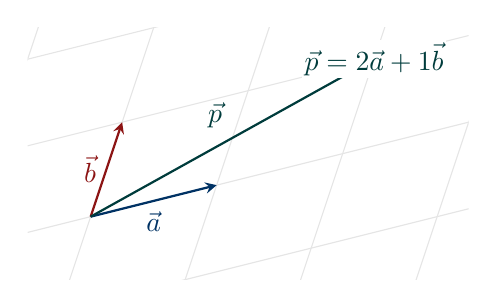
\begin{tikzpicture}[scale=0.8, >=stealth]
        \clip (-1,-1) rectangle (6,3);
        \coordinate (O) at (0,0);
        \coordinate (A) at (2,0.5);   % vec a
        \coordinate (B) at (0.5,1.5); % vec b
        
        % グリッド線 (修正箇所: スカラー倍は $s*(A)$ のように係数を前に書く)
        \foreach \s in {-2,-1,...,5} {
            \draw[gray!20] ($ \s*(A) - 2*(B) $) -- ($ \s*(A) + 4*(B) $);
        }
        \foreach \t in {-2,-1,...,5} {
            \draw[gray!20] ($ \t*(B) - 2*(A) $) -- ($ \t*(B) + 5*(A) $);
        }
        
        % ベクトル
        \draw[->, thick, printBlue] (O) -- (A) node[midway, below] {$\vec{a}$};
        \draw[->, thick, printRed] (O) -- (B) node[midway, left] {$\vec{b}$};
        
        % 点Pの例 (2a + b) (修正箇所)
        \coordinate (P) at ($ 2*(A) + 1*(B) $);
        \fill (P) circle (2pt) node[right] {P};
        \draw[->, thick, printTeal] (O) -- (P) node[midway, above left] {$\vec{p}$};
        \node[printTeal, fill=white, inner sep=1pt] at (4.5, 2.5) {$\vec{p} = 2\vec{a} + 1\vec{b}$};
    \end{tikzpicture}
    \end{center}
    どんな場所にある点Pも, 基底の足し合わせで表現できる.
\end{any}

%-----------------------------------------------------------------------------
% 右カラム:分解の一意性
%-----------------------------------------------------------------------------
\columnbreak

\begin{any}{2. ベクトルの分解定理}
    \begin{thm}{分解の一意性(最重要)}
        $\vec{a}, \vec{b}$ が一次独立であるとき, 平面上の\textbf{任意のベクトル} $\vec{p}$ は, 実数 $s, t$ を用いて
        \[ \vec{p} = s\vec{a} + t\vec{b} \]
        の形に\textbf{ただ1通りに}表される.
    \end{thm}

    \begin{eg}{1 (図形の分解)}
        平行四辺形ABCDにおいて, 辺BCの中点をM, 辺CDの中点をNとする. $\overrightarrow{\text{AB}}=\vec{a}, \overrightarrow{\text{AD}}=\vec{b}$ とするとき, $\overrightarrow{\text{AM}}, \overrightarrow{\text{AN}}$ を $\vec{a}, \vec{b}$ で表せ.
        
        \tcblower
        \begin{center}
        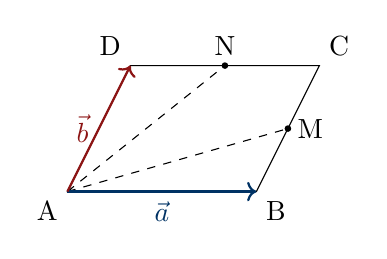
\begin{tikzpicture}[scale=0.8]
            \coordinate (A) at (0,0);
            \coordinate (B) at (3,0);
            \coordinate (D) at (1,2);
            \coordinate (C) at (4,2);
            \coordinate (M) at (3.5, 1);
            \coordinate (N) at (2.5, 2);
            
            \draw (A)--(B)--(C)--(D)--cycle;
            \draw[dashed] (A)--(M) (A)--(N);
            \fill (M) circle (1.5pt) node[right] {M};
            \fill (N) circle (1.5pt) node[above] {N};
            \node[below left] at (A) {A};
            \node[below right] at (B) {B};
            \node[above right] at (C) {C};
            \node[above left] at (D) {D};
            
            \draw[->, thick, printBlue] (A)--(B) node[midway, below] {$\vec{a}$};
            \draw[->, thick, printRed] (A)--(D) node[midway, left] {$\vec{b}$};
        \end{tikzpicture}
        \end{center}
        \vspace{3cm} % 記述スペース
    \end{eg}
\end{any}

\end{multicols}

%=============================================================================
% 2枚目:係数比較法
%=============================================================================
\newpage
\begin{multicols}{2}

%-----------------------------------------------------------------------------
% 左カラム:係数比較
%-----------------------------------------------------------------------------
\begin{any}{3. 係数比較法}
    分解が「1通り」しかないため, 係数を比較して方程式を作ることができる.

    \begin{thm}{係数比較の定理}
        $\vec{a}, \vec{b}$ が一次独立であるとき,
        \begin{enumerate}
            \item $s\vec{a} + t\vec{b} = \vec{0} \iff s=0 \text{ かつ } t=0$
            \item $s\vec{a} + t\vec{b} = s'\vec{a} + t'\vec{b} \iff s=s' \text{ かつ } t=t'$
        \end{enumerate}
    \end{thm}
    
    \textbf{記述上の注意:} \\
    この定理を使うときは, 必ず\textbf{「$\vec{a} \neq \vec{0}, \vec{b} \neq \vec{0}, \vec{a} \not\parallel \vec{b}$ なので」}(または単に「$\vec{a}, \vec{b}$ は一次独立なので」)という断り書きが必要である.
\end{any}

\begin{eg}{2 (係数決定)}
    $\vec{a}, \vec{b}$ は一次独立とする.
    \[ (3x + y)\vec{a} + (x - 2y - 7)\vec{b} = \vec{0} \]
    を満たす実数 $x, y$ の値を求めよ.
    \tcblower
    \vspace{6cm} 
\end{eg}

%-----------------------------------------------------------------------------
% 右カラム:分解の応用
%-----------------------------------------------------------------------------
\columnbreak

\begin{eg}{3 (基底の変換)}
    $\vec{a}, \vec{b}$ は一次独立とする.
    $\vec{p} = 2\vec{a} + 3\vec{b}$, $\vec{q} = \vec{a} - 2\vec{b}$ であるとき,
    $\vec{a}$ を $\vec{p}, \vec{q}$ を用いて表せ.
    
    \tcblower
    \textbf{方針:} 連立方程式のように $\vec{b}$ を消去する.
    \vspace{8cm} 
\end{eg}

\end{multicols}

%=============================================================================
% 3枚目:確認テスト(問題)
%=============================================================================
\newpage
\fancyhead[L]{\small \textcolor{black!90}{数学C $>$ 第1章--平面ベクトル $>$ 第2回--\textbf{確認テスト}}}
\begin{multicols}{2}

\begin{any}{確認テスト (A: 基本)}
    \begin{prac}{A1 (図形の分解)}
        平行四辺形ABCDの対角線の交点をOとする. $\overrightarrow{\text{OA}}=\vec{a}, \overrightarrow{\text{OB}}=\vec{b}$ とするとき, 次のベクトルを $\vec{a}, \vec{b}$ で表せ.
        \begin{enumerate}
            \item $\overrightarrow{\text{OC}}$
            \item $\overrightarrow{\text{AB}}$
            \item $\overrightarrow{\text{BC}}$
        \end{enumerate}
        
        \begin{center}
        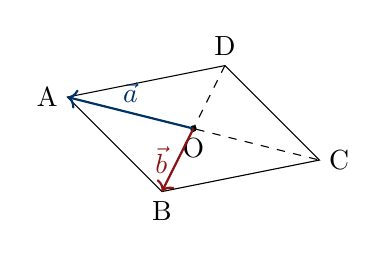
\begin{tikzpicture}[scale=0.8]
            \coordinate (O) at (0,0);
            \coordinate (A) at (-2,0.5);
            \coordinate (B) at (-0.5,-1);
            \coordinate (C) at (2,-0.5);
            \coordinate (D) at (0.5,1);
            
            \draw (A)--(B)--(C)--(D)--cycle;
            \draw[dashed] (A)--(C) (B)--(D);
            \fill (O) circle (1.5pt) node[below] {O};
            \node[left] at (A) {A}; \node[below] at (B) {B};
            \node[right] at (C) {C}; \node[above] at (D) {D};
            
            \draw[->, thick, printBlue] (O)--(A) node[midway, above] {$\vec{a}$};
            \draw[->, thick, printRed] (O)--(B) node[midway, left] {$\vec{b}$};
        \end{tikzpicture}
        \end{center}
    \end{prac}
    
    \begin{answer}[height=3cm]
    \end{answer}

    \begin{prac}{A2 (係数比較)}
        $\vec{a}, \vec{b}$ は一次独立とする.
        \[ (x-2)\vec{a} + (2x+y-5)\vec{b} = \vec{0} \]
        を満たす実数 $x, y$ を求めよ.
    \end{prac}

    \begin{answer}[height=3cm]
    \end{answer}
\end{any}

\columnbreak

\begin{any}{確認テスト (B: 標準)}
    \begin{prac}{B1 (基底の変換)}
        $\vec{a}, \vec{b}$ は一次独立とする. 
        \[ \vec{u} = 2\vec{a} - \vec{b}, \quad \vec{v} = -\vec{a} + 3\vec{b} \]
        であるとき, $\vec{p} = 3\vec{a} + \vec{b}$ を $\vec{u}, \vec{v}$ を用いて表せ.
    \end{prac}

    \begin{answer}[height fill]
    \end{answer}
\end{any}

\end{multicols}

%=============================================================================
% 4枚目:確認テスト(解答)
%=============================================================================
\newpage
\fancyhead[L]{\small \textcolor{black!90}{数学C $>$ 第1章--平面ベクトル $>$ 第2回 \textbf{【解答解説】}}}

\begin{multicols}{2}

\begin{any}{解答 (A: 基本)}
    \begin{prac}{A1 (図形の分解)}
        (1) OはACの中点. $\overrightarrow{\text{OC}}$ は $\overrightarrow{\text{OA}}$ の逆ベクトル.
        \[ \overrightarrow{\text{OC}} = -\overrightarrow{\text{OA}} = \boldsymbol{-\vec{a}} \]
        (2) 終点 $-$ 始点.
        \[ \overrightarrow{\text{AB}} = \overrightarrow{\text{OB}} - \overrightarrow{\text{OA}} = \boldsymbol{\vec{b} - \vec{a}} \]
        (3) $\overrightarrow{\text{BC}} = \overrightarrow{\text{OC}} - \overrightarrow{\text{OB}} = (-\vec{a}) - \vec{b} = \boldsymbol{-\vec{a} - \vec{b}}$
    \end{prac}

    \begin{answer}[height=8cm]
    \color{printRed}
    \textbf{A2 解答:} \\
    $\vec{a}, \vec{b}$ は一次独立なので, 係数はそれぞれ $0$ である.
    \[
    \begin{cases}
        x - 2 = 0 \\
        2x + y - 5 = 0
    \end{cases}
    \]
    第1式より $x = 2$. 第2式に代入して $4 + y - 5 = 0 \iff y = 1$. \\
    \textbf{答え:} $x=2, y=1$
    \end{answer}
\end{any}

\columnbreak

\begin{any}{解答 (B: 標準)}
    \begin{answer}[height fill]
    \color{printRed}
    \textbf{B1 解答:} \\
    $\vec{p} = s\vec{u} + t\vec{v}$ とおき, $s, t$ を決定する(係数比較法).
    
    代入して整理すると:
    \begin{align*}
        \vec{p} &= s(2\vec{a} - \vec{b}) + t(-\vec{a} + 3\vec{b}) \\
        &= (2s - t)\vec{a} + (-s + 3t)\vec{b}
    \end{align*}
    一方で, 問題の条件より $\vec{p} = 3\vec{a} + \vec{b}$ である.
    $\vec{a}, \vec{b}$ は一次独立であるから, 係数を比較して:
    \[
    \begin{cases}
        2s - t = 3 & \cdots (1) \\
        -s + 3t = 1 & \cdots (2)
    \end{cases}
    \]
    (2)より $s = 3t - 1$. これを(1)に代入.
    $2(3t - 1) - t = 3 \implies 6t - 2 - t = 3 \implies 5t = 5 \implies t = 1$.
    よって $s = 3(1) - 1 = 2$.
    
    したがって,
    \[ \boldsymbol{\vec{p} = 2\vec{u} + \vec{v}} \]
    
    \textbf{別解(連立方程式として解く):} \\
    $\vec{u} = 2\vec{a} - \vec{b} \dots (i)$ \\
    $\vec{v} = -\vec{a} + 3\vec{b} \dots (ii)$ \\
    $(i) + 2 \times (ii)$ より $\vec{u} + 2\vec{v} = 5\vec{b} \implies \vec{b} = \frac{1}{5}(\vec{u} + 2\vec{v})$. \\
    同様に $\vec{a}$ を $\vec{u}, \vec{v}$ で表して $\vec{p}$ に代入してもよい.
    \end{answer}
\end{any}

\end{multicols}
\end{document}